
%%% Local Variables:
%%% mode: latex
%%% TeX-master: t
%%% End:

\chapter{基于AS编址的互联网可扩展路由机制的仿真评价}
\label{cha:simu}
\section{引言}
本章将讨论如何对基于AS编址的互联网可扩展路由机制的仿真评价,主要包括以下内容:仿真实验平台SIMBGP的介绍,仿真实验的过程以及结果分析。选取SIMBGP作为我们仿真实验的工具,分别统计和分析自治系统宣布CABA编址下的一条前缀和宣布多条现今网络宣布出去的前缀到互联网中,在网络路由信息稳定之后,互联网宣布的UPDATE 条数和收敛时间。

\section{仿真实验平台介绍}
\subsection{平台特点及运行方法}
\begin{itemize}
\item 平台特点:SIMBGP是一个超轻量级的BGP协议仿真器,忽略了所有底层的协议;该平台使用Python 语言实现,只有一个文件,运行简单;该平台可以在互联网的全网拓扑结构上进行仿真,满足实验要求;SIMBGP是一个事件驱动型的模拟器,使用者可以很容易的了解代码的结构以及在运行的过程中容易监控程序运行的程度,但是这也就意味着该仿真平台是单进程,向外宣布前缀只能一条一条向外宣布,不能同时执行多个事件,影响了批量模拟ANNOUNCE事件的效率。
\item 运行方法:在linux系统的terminal窗口运行python simbgp.py  config.txt,运行需要输入BGP配置文件,表示网络的拓扑结构。
\end{itemize}

\subsection{配置文件}
\label{subsect:config}
仿真实验需要在全网的拓扑结构下进行,所以要生成表示全网拓扑结构关系的配置文件,大致可以分为两步:
第一步:获取自治系统间的拓扑结构,自治系统的关系来自于CAIDA官网上的数据\onlinecite{caidaasdata}。下载获得的数据部分如下:\\
1267$|$60280$|$-1\\
1267$|$20756$|$0

解读自治系统关系的文件需要参考文件\onlinecite{caidaasreadme},该格式的含义如下:\\
$<$provider-as$>|<$customer-as$>|$-1\\
$<$peer-as$>|<$peer-as$>|$0

第二步:为了简化拓扑结构,以自治系统为最小单位,每台路由器为一个自治系统。编写程序遵循SIMBGP的配置文件格式生成配置文件。

\section{仿真实验流程设计}
SIMBGP仿真实验的流程如下:
\begin{itemize}
\item 从CAIDA官网获得全网的拓扑结构,编写程序生成SIMBGP的输入配置文件,参考\ref{subsect:config}。
\item 在本文\ref{sect:fibtab}章节获得了saopaulo路由器的当前网络下FIB表数据,统计每个自治系统公布出去的前缀。
\item 在全网约50000自治系统中随机选取20个自治系统号。
\item 自治系统A宣布嵌入自治系统号A的ipv6前缀,获取UPDATE数目和收敛时间。
\item 自治系统A宣布saopaulo路由器的当前网络下FIB表数据中公布出去的所有前缀,统计UPDATE数目和收敛时间。
\end{itemize}

\section{仿真实验结果分析}



\begin{table}[h]
  \centering
  \caption{SIMBGP仿真实验结果}
  \label{tab:simres}
  \begin{tabular}{|c|c|c|c|c|}
            \hline
            随机ASN & 现今网络中宣告Prefix数目 & UPDATE条数 & 收敛时间 & UPDATE减少倍数\\ \hline
            393393 & 17 & 445622 & 134.17 & 16 \\ \hline
            21021 & 32 & 436523 & 90.02 & 32 \\ \hline
            45773 & 53 & 514378 & 118.14 & 52 \\ \hline
            29684 & 73 & 490768 & 117.37 & 72 \\ \hline
            9535 & 114 & 506102 & 114.34 & 113 \\ \hline
            11003 & 121 & 475602 & 114.21 & 120 \\ \hline
            18978 & 144 & 434848 & 109.3 & 143 \\ \hline
            38370 & 174 & 460682 & 100.59 & 173 \\ \hline
            12418 & 189 & 449055 & 109.16 & 188 \\ \hline
            20299 & 216 & 512391 & 134.02 & 215 \\ \hline
            23674 & 260 & 496074 & 118.15 & 259 \\ \hline
            702 & 284 & 410536 & 106.48 & 283 \\ \hline
            3491 & 337 & 437333 & 90.87 & 336 \\ \hline
            812 & 403 & 422310 & 88.1 & 402 \\ \hline
            17762 & 453 & 460750 & 107.77 & 452 \\ \hline
            18207 & 595 & 468700 & 115.25 & 594 \\ \hline
            11139 & 619 & 419390 & 89.65 & 618 \\ \hline
            15003 & 839 & 440663 & 112.17 & 838 \\ \hline
            13188 & 1102 & 448425 & 111.64 & 1101 \\ \hline
            22394 & 1486 & 425741 & 110.53 & 1485 \\ \hline
            平均值 & 375.55 & 457795 & 109.60 & 375 \\ \hline
  \end{tabular}
\end{table}


SIMBGP仿真实验的结果如表\ref{tab:simres}所示,对其结果进行分析:
在仿真实验中,通过一台路由器代表一个自治系统,在这个自治系统中prefix只是一个标签,所以路由器向外宣告一条CABA编址下的前缀和向外宣告一条现今网络宣告出去的IPv4\/IPv6路由所宣布的UPDATE数目相同,所需要的收敛时间也是相同的。
平均减少的update条数有45万$*$300$=1.35*10^{8}$,约减少300倍,收敛时间大部分为100s。

\begin{figure}
  \centering
  % Requires \usepackage{graphicx}
  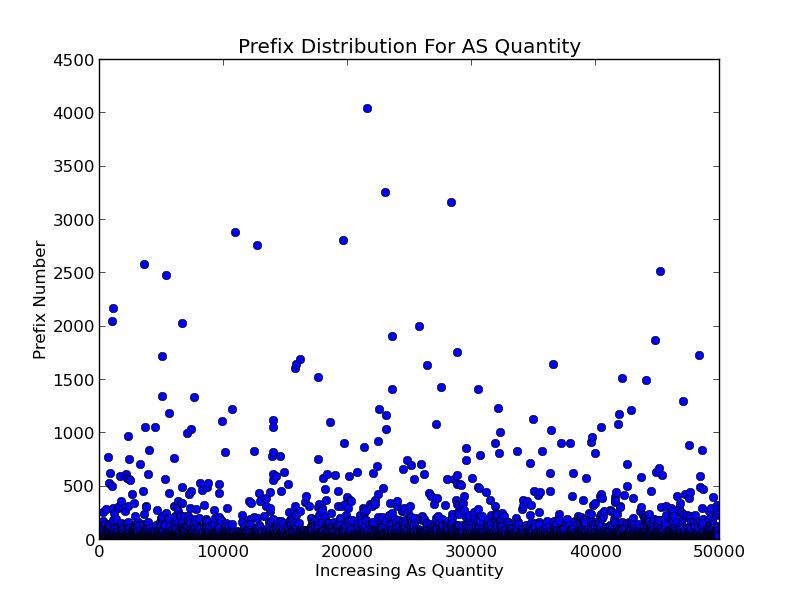
\includegraphics[width=\textwidth]{asnprefix}\\
  \caption{ASN对应宣告前缀数目的散点图}\label{fig:asnprefix}
\end{figure}

\begin{figure}
  \centering
  % Requires \usepackage{graphicx}
  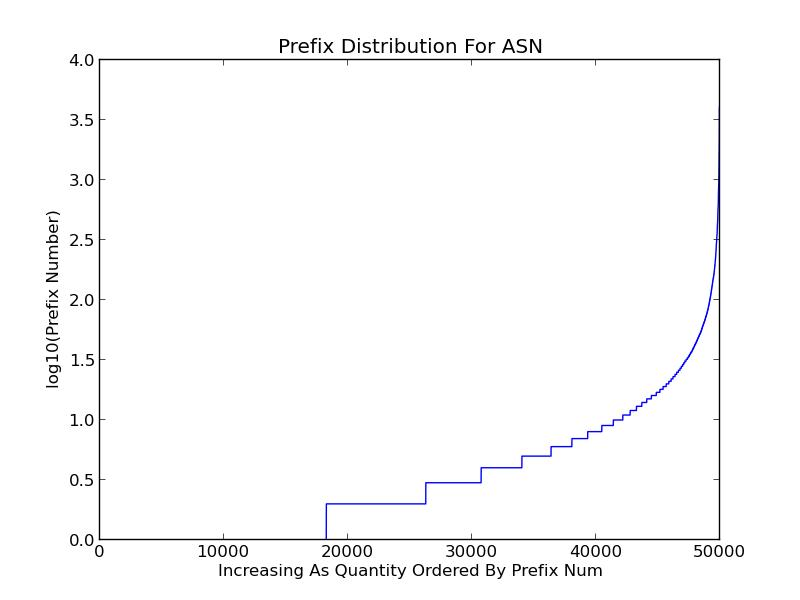
\includegraphics[width=\textwidth]{7}\\
  \caption{宣告前缀数目递增的ASN对应宣告前缀数目的LOG值}\label{fig:7}
\end{figure}

\begin{figure}
  \centering
  % Requires \usepackage{graphicx}
  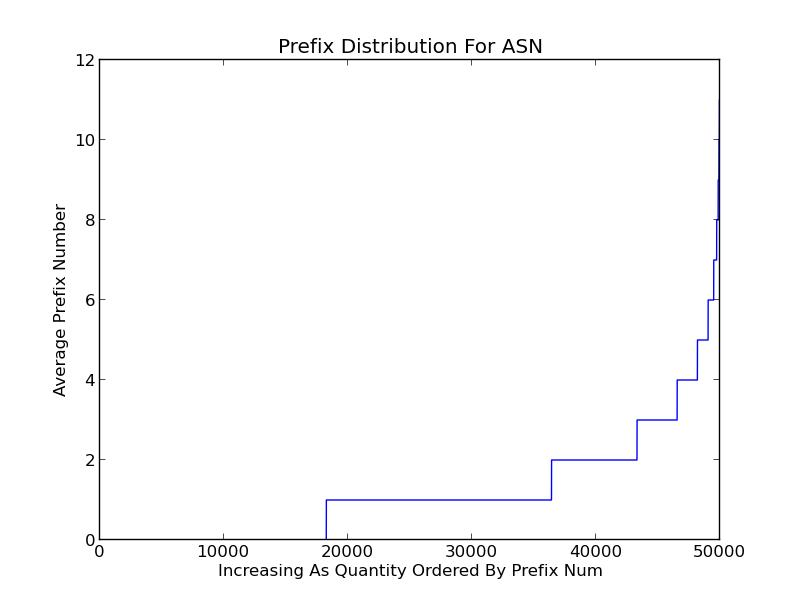
\includegraphics[width=\textwidth]{6}\\
  \caption{宣告前缀数目递增的ASN对应的平均宣告前缀数目的CDF图}\label{fig:6}
\end{figure}

可以观测到,CABA编址下宣告前缀比现今网络下宣告前缀之间,UPDATE数目差异主要和自治系统在现今网络下向外宣布的前缀数目相关。
由图\ref{fig:asnprefix}可得,AS对应的前缀数目聚集在1-500之间,在0-200最为密集。

由图\ref{fig:7}可以看出有1万多个自治系统只向外宣告了一个前缀,有4万多个前缀系统向外宣告了小于10个前缀,也就是说对于大部分的自治系统而言,部署CABA地址分配方案,向外宣布嵌有ASN的直到网络路由收敛的UPDATE的数目和没有部署向外宣布现今网络中的前缀直到网络路由收敛的UPDATE数目相比,并没有很大程度的减少。

由图\ref{fig:6}可以看出一个自治系统平均向外宣布10条前缀,部署CABA地址分配方案的自治系统,向外宣布嵌有ASN的直到网络路由收敛的UPDATE 的数目平均是没有部署向外宣布现今网络中的前缀直到网络路由收敛的UPDATE数目的$1/10$。



\section{小结}
综上所述,一个自治系统平均向外宣布10条前缀,部署CABA地址分配方案的自治系统,向外宣布嵌有ASN的直到网络路由收敛的UPDATE 的数目平均是没有部署向外宣布现今网络中的前缀直到网络路由收敛的UPDATE数目的$1/10$。部署CABA方案的自治系统只需要向外宣布一条前缀,与现今网络中一个自治系统需要向外宣告n条前缀相比,update减少$(n-1)/n$。所以,部署CABA方案在向外宣布较多前缀的自治系统上,更有利于减少BGP路由信息的交互。

